\textbf{Partial Differential Equations (PDEs)}\\
\begin{wrapfigure}{r}{.3\textwidth}
        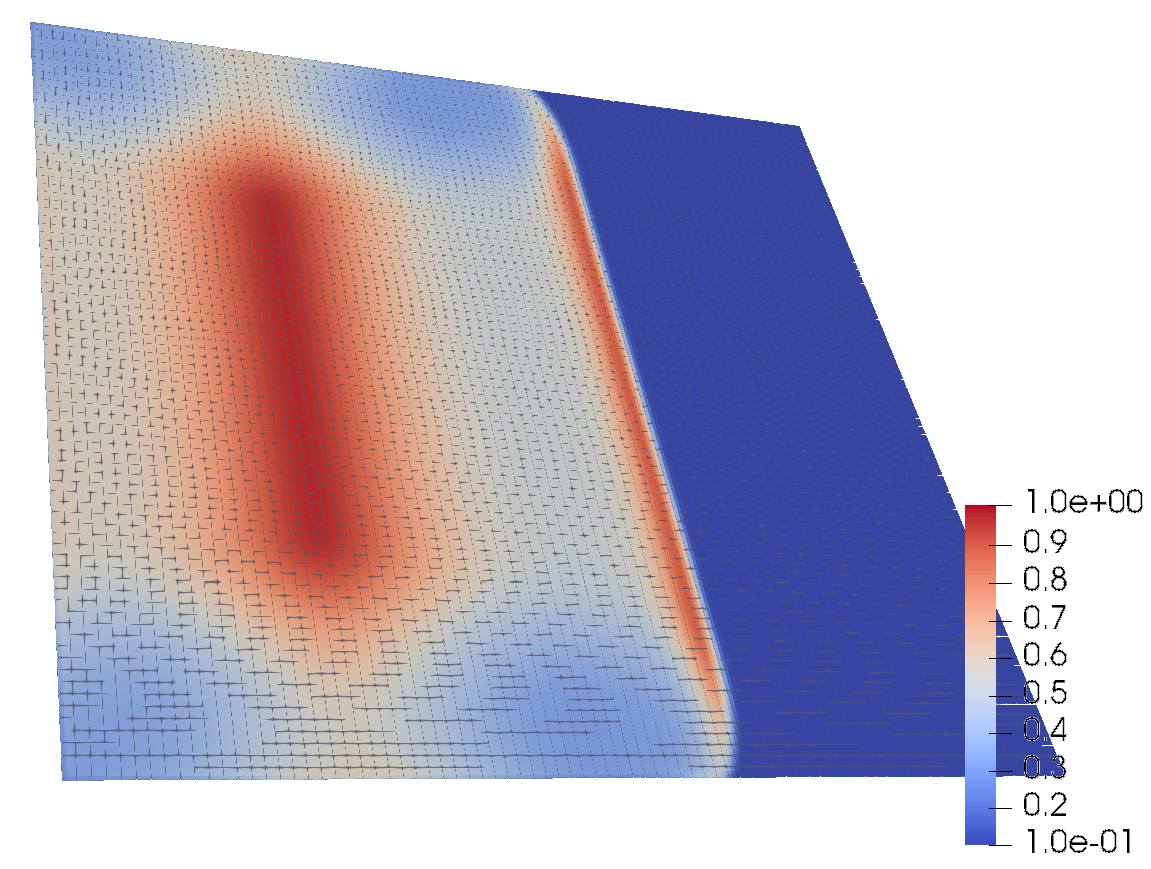
\includegraphics[width=.3
        \textwidth]{PDE-pick-2.png}
\end{wrapfigure}
It is often more natural to describe how a system changes as opposed to a systems absolute state, and this is what PDEs do.
PDEs are ubiquitous in describing the world around us, describing 
phenomena such as seismic waves and fluid mechanics.
However, it is often impossible to find an analytical solution to PDEs, hence we rely 
on numerical schemes such as Finite Volumes (FV) to calculate approximate 
solutions.
Calculating a solution with sufficient accuracy for a large problem is very computationally intensive, requiring billions of degrees of freedom and often the use of supercomputers

\phantom{ }

\textbf{ExaHyPE}\\
ExaHyPE (``An Exascale Hyperbolic PDE Engine'') is a software engine for solving systems of first-order hyperbolic PDEs \cite{exahype}.
ExaHyPE enables users to create highly sophisticated PDE solvers with ease, 
supporting complex features such as adaptive mesh sizing while scaling well across 
super computing hardware.
To make an ExaHyPE programs a user describes their problem to the ExaHyPE toolkit, which then generates a template program.
A user then fills in placeholder functions that calculate problem specific quantities such as eignen values.
Then the program is ready to be compiled and run, working on hardware ranging from a laptop to exa-scale supercomputers.



